\documentclass[11pt]{beamer} % mathserif for normal math fonts.
\usefonttheme[onlymath]{serif}
\usepackage[utf8]{inputenc}
\usepackage[swedish,english]{babel}
\usepackage{amsmath,mathtools}
\usepackage{calc}
\usepackage{minted}

\usepackage[T1]{fontenc}

% The Chalmers theme:
\usetheme[titleflower=true]{chalmers} % titleflower = true or false
\title{Stack Traces in Haskell}
% \subtitle{And something more} % optional % I dont need it /Arash
\author[Arash Rouhani]{Arash Rouhani} % [short author (optional)]{many authors}
\institute{Chalmers University of Technology}
\titlepageextra{Master thesis presentation} % Optional extra info, appears before date on title page
\footer{\insertshortauthor\ -- Thesis presentation} % optional, manually sets footer (default is short author)
%\footer{Something completely different} % but it can of course be anything.
\titlepagelogofile{figures/Avancez_black} % File name to the file you want to include.
%\titlepagelogo{\tikz{\draw(0,0) circle (1);}} % or draw anything for a logo


% https://3diagramsperpage.wordpress.com/2013/10/26/template-for-code-highlighting-with-minted-in-latex-beamer/
% http://alturl.com/689br
\newminted{haskell}{fontsize=\scriptsize,
		   linenos,
		   numbersep=8pt,
		   gobble=2,
		   frame=lines,
		   bgcolor=bg,
		   framesep=3mm
       }

\newminted{text}{fontsize=\scriptsize,
		   gobble=2,
		   bgcolor=bg
		   }


\begin{document}
% http://alturl.com/689br
\definecolor{bg}{rgb}{0.95,0.95,0.95}

% http://alturl.com/689br
\defverbatim[colored]\exampleCode{
\begin{haskellcode}
  hi = world

\end{haskellcode}
}

\defverbatim[colored]\motivationCode{
\begin{haskellcode}
  main = print (f 10)
  f x = ... g y ...
  g x = ... h y ...
  h x = ... head [] ...

\end{haskellcode}
}

\defverbatim[colored]\outputNoTrace{
\begin{textcode}
  $ runghc Crash.hs
  Crash.hs: Prelude.head: empty list
\end{textcode}
}

\defverbatim[colored]\outputTrace{
\begin{textcode}
  $ runghc Crash.hs
  Crash.hs: Prelude.head: empty list
    in function   h
    in function   g
    in function   f
    in function   main
\end{textcode}
}

\defverbatim[colored]\lazyCode{
\begin{haskellcode}
  myIf :: Bool -> a -> a -> a
  myIf True  x y = x
  myIf False x y = y

  -- Then evaluate
  myIf True 5 (error "evil crash")

\end{haskellcode}
}

\defverbatim[colored]\caseCode{
\begin{haskellcode}
  case myBool of
    True  -> this
    False -> that
\end{haskellcode}
}

\defverbatim[colored]\useGhcCode{
\begin{textcode}
  $ ghc --make Code.hs
  ...
  $ ./a.out
  123
\end{textcode}
}

\defverbatim[colored]\getDebugInfoCode{
\begin{haskellcode}
  getDebugInfo :: Ptr Instruction -- Pointer to runnable machine code
               -> IO DebugInfo -- Haskell function name etc.
\end{haskellcode}
}

\defverbatim[colored]\dwarfCode{
\begin{textcode}
  < 1><0x0000008d>    DW_TAG_subprogram
                        DW_AT_name                  "addition"
                        DW_AT_MIPS_linkage_name     "r8m_info"
                        DW_AT_external              no
                        DW_AT_low_pc                0x00000020
                        DW_AT_high_pc               0x00000054
                        DW_AT_frame_base            DW_OP_call_frame_cfa
  < 2><0x000000b3>      DW_TAG_lexical_block
                          DW_AT_name                  "cmG_entry"
                          DW_AT_low_pc                0x00000029
                          DW_AT_high_pc               0x0000004b
  < 2><0x000000cf>      DW_TAG_lexical_block
                          DW_AT_name                  "cmF_entry"
                          DW_AT_low_pc                0x0000004b
                          DW_AT_high_pc               0x00000054
\end{textcode}
}

\defverbatim[colored]\HaskellSTCode{
\begin{haskellcode}
  main :: IO ()
  main = do a
            print 2

  a, b :: IO ()
  a = do b
         print 20

  b = do print (crashSelf 2)
         print 200

  crashSelf :: Int -> Int
  crashSelf 0 = 1 `div` 0
  crashSelf x = crashSelf (x - 1)
\end{haskellcode}
}

\defverbatim[colored]\OriginalTraceCode{
\begin{textcode}
   0: stg_bh_upd_frame_ret
   1: stg_bh_upd_frame_ret
   2: stg_bh_upd_frame_ret
   3: showSignedInt
   4: stg_upd_frame_ret
   5: writeBlocks
   6: stg_ap_v_ret
   7: bindIO
   8: bindIO
   9: bindIO
  10: stg_catch_frame_ret
\end{textcode}
}

\defverbatim[colored]\IdealTraceCode{
\begin{textcode}
   0: crashSelf
   1: crashSelf
   2: print
   3: b
   4: a
   5: main
\end{textcode}
}

\defverbatim[colored]\obviouslyThunkCode{
\begin{haskellcode}
  powerTwo :: Int -> Int
  powerTwo 0 = 1
  powerTwo n = x + x
    where x = powerTwo (n - 1)
\end{haskellcode}
}

\defverbatim[colored]\improvedTraceCode{
\begin{textcode}
   0: stg_bh_upd_frame_ret   ----------->      0: divZeroError
   1: stg_bh_upd_frame_ret   ----------->      1: crashSelf
   2: stg_bh_upd_frame_ret   ----------->      2: b
   3: showSignedInt          ----------->      3: showSignedInt
   4: stg_upd_frame_ret      ----------->      4: print
   5: writeBlocks            ----------->      5: writeBlocks
   6: stg_ap_v_ret           ----------->      6: stg_ap_v_ret
   7: bindIO                 ----------->      7: bindIO
   8: bindIO                 ----------->      8: bindIO
   9: bindIO                 ----------->      9: bindIO
  10: stg_catch_frame_ret    ----------->     10: stg_catch_frame_ret
\end{textcode}
}


\defverbatim[colored]\catchWithStackCode{
\begin{haskellcode}
  catchWithStack :: Exception e =>
         IO a                 -- Action to run
      -> (e -> Stack -> IO a) -- Handler
      -> IO a
\end{haskellcode}
}

%\setlength{\footertextwidth}{0.5\paperwidth} % You might need to adjust this if the text doesn't fit well.

\section{Title page} % Sections are shown at the bottom left. There is also links in many pdf-readers
\begin{frame}[plain]
 \titlepage
\end{frame}

\section{Contents}
\begin{frame}
 \frametitle{Contents}
 % \framesubtitle{With subtitle}
\begin{itemize}
 \item Motivation
 \item Background
 \item The attempt in August 2013
 \item Contribution
\end{itemize}
\end{frame}

\section{Motivation}

  \begin{frame}
   \frametitle{An old problem \dots}
  \begin{itemize}
   \item <1-> Try running this program:
     \motivationCode
   \item <2-> You get
     \outputNoTrace
   \item <3-> But you want
     \outputTrace
  \end{itemize}
  \end{frame}

  \begin{frame}
   \frametitle{\dots with new constraints}
  \begin{itemize}
   \item Should have very low overhead
   \item If you hesitate to use it in production, I've failed
   \item Not done for Haskell before, all earlier work have an overhead.
  \end{itemize}
  \end{frame}

\section{Background}

  \begin{frame}
   \frametitle{Background contents}
  \begin{itemize}
   \item Is stack traces harder for \emph{Haskell}?
   \item Will the implementation only work for \emph{GHC}?
  \end{itemize}
  \end{frame}


\subsection{Haskell}

  \begin{frame}
   \frametitle{Laziness}
  \begin{itemize}
   \item <1-> Consider the code
     \lazyCode
   \item <1-> Will the usage of \texttt{error} make this crash?
   \item <2-> No, \texttt{(error "evil crash")} is a \emph{delayed computation}.
  \end{itemize}
  \end{frame}

  \begin{frame}
   \frametitle{Case expressions}
  \begin{itemize}
   \item <1-> Consider the code
     \caseCode
   \item <1-> So is pattern matching just like \texttt{switch-case} in C?
   \item <2-> NO!
   \item <3-> \texttt{myBool} can be a delayed computation, aka a \emph{thunk}
  \end{itemize}
  \end{frame}

\subsection{GHC}
  \begin{frame}
   \frametitle{History of GHC}
  \begin{itemize}
   \item Compiles Haskell to machine code since 1989
   \item The only Haskell compiler people care about
  \end{itemize}
  \end{frame}

  \begin{frame}
   \frametitle{Usage}
  \begin{itemize}
   \item Compile and run (just like any other compiler)
     \useGhcCode
  \end{itemize}
  \end{frame}

\subsubsection{Magic function}
  \begin{frame}
   \frametitle{The magical function}
  \begin{itemize}
   \item <1-> My work assumes the existence of
     \getDebugInfoCode
   \item <2-> This is a recent contribution not yet merged in HEAD 
   \item <2-> Author is
     \href{http://www.personal.leeds.ac.uk/~scpmw/site.html}{Peter Wortmann},
     part of his PhD at Leeds
   \item <3-> \emph{In essence, 95\% of the job to implement stack traces was
       already done!}
  \end{itemize}
  \end{frame}

  \begin{frame}
   \frametitle{The compilation pipeline}
  \begin{itemize}
   \item <1-> Well GHC works like this:
     \includegraphics[width=4in]{build/fig/ghc}
   \item <2-> Or rather like this
     \includegraphics[width=4in]{build/fig/phases}
   \item <3-> We say that GHC has many \emph{Intermediate Representations}
  \end{itemize}
  \end{frame}

  \begin{frame}
   \frametitle{So there must be debug data!}
  \begin{itemize}
   \item <1-> Again:
     \includegraphics[width=4in]{build/fig/ghc}
   \item <2-> The intuition behind \texttt{getDebugInfo} is:
     \includegraphics[width=4in]{build/fig/ghc-reverse}
   \item <3-> For this, we \emph{must} retain debug data in the binary!
  \end{itemize}
  \end{frame}

  \begin{frame}
   \frametitle{Lets get to work!}
   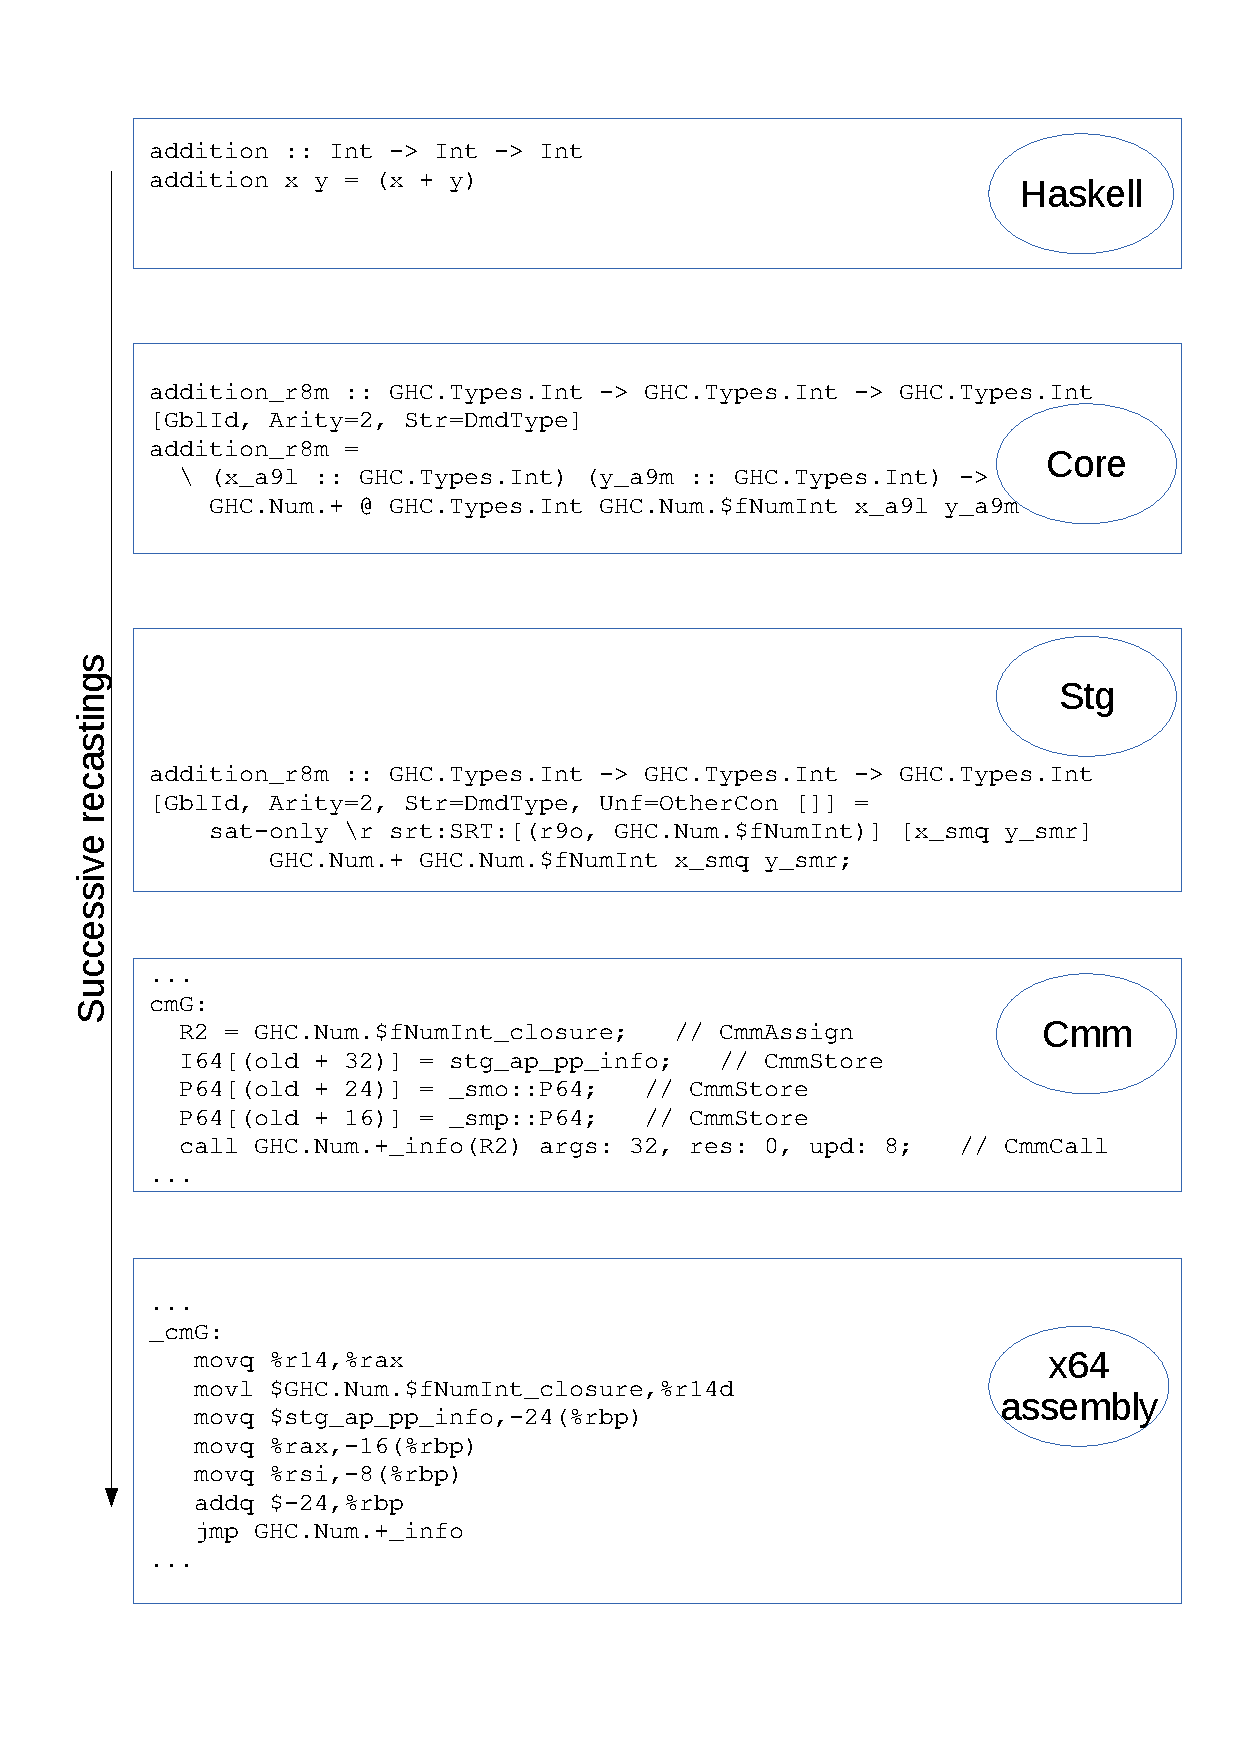
\includegraphics[width=2.2in]{fig/recastings}
   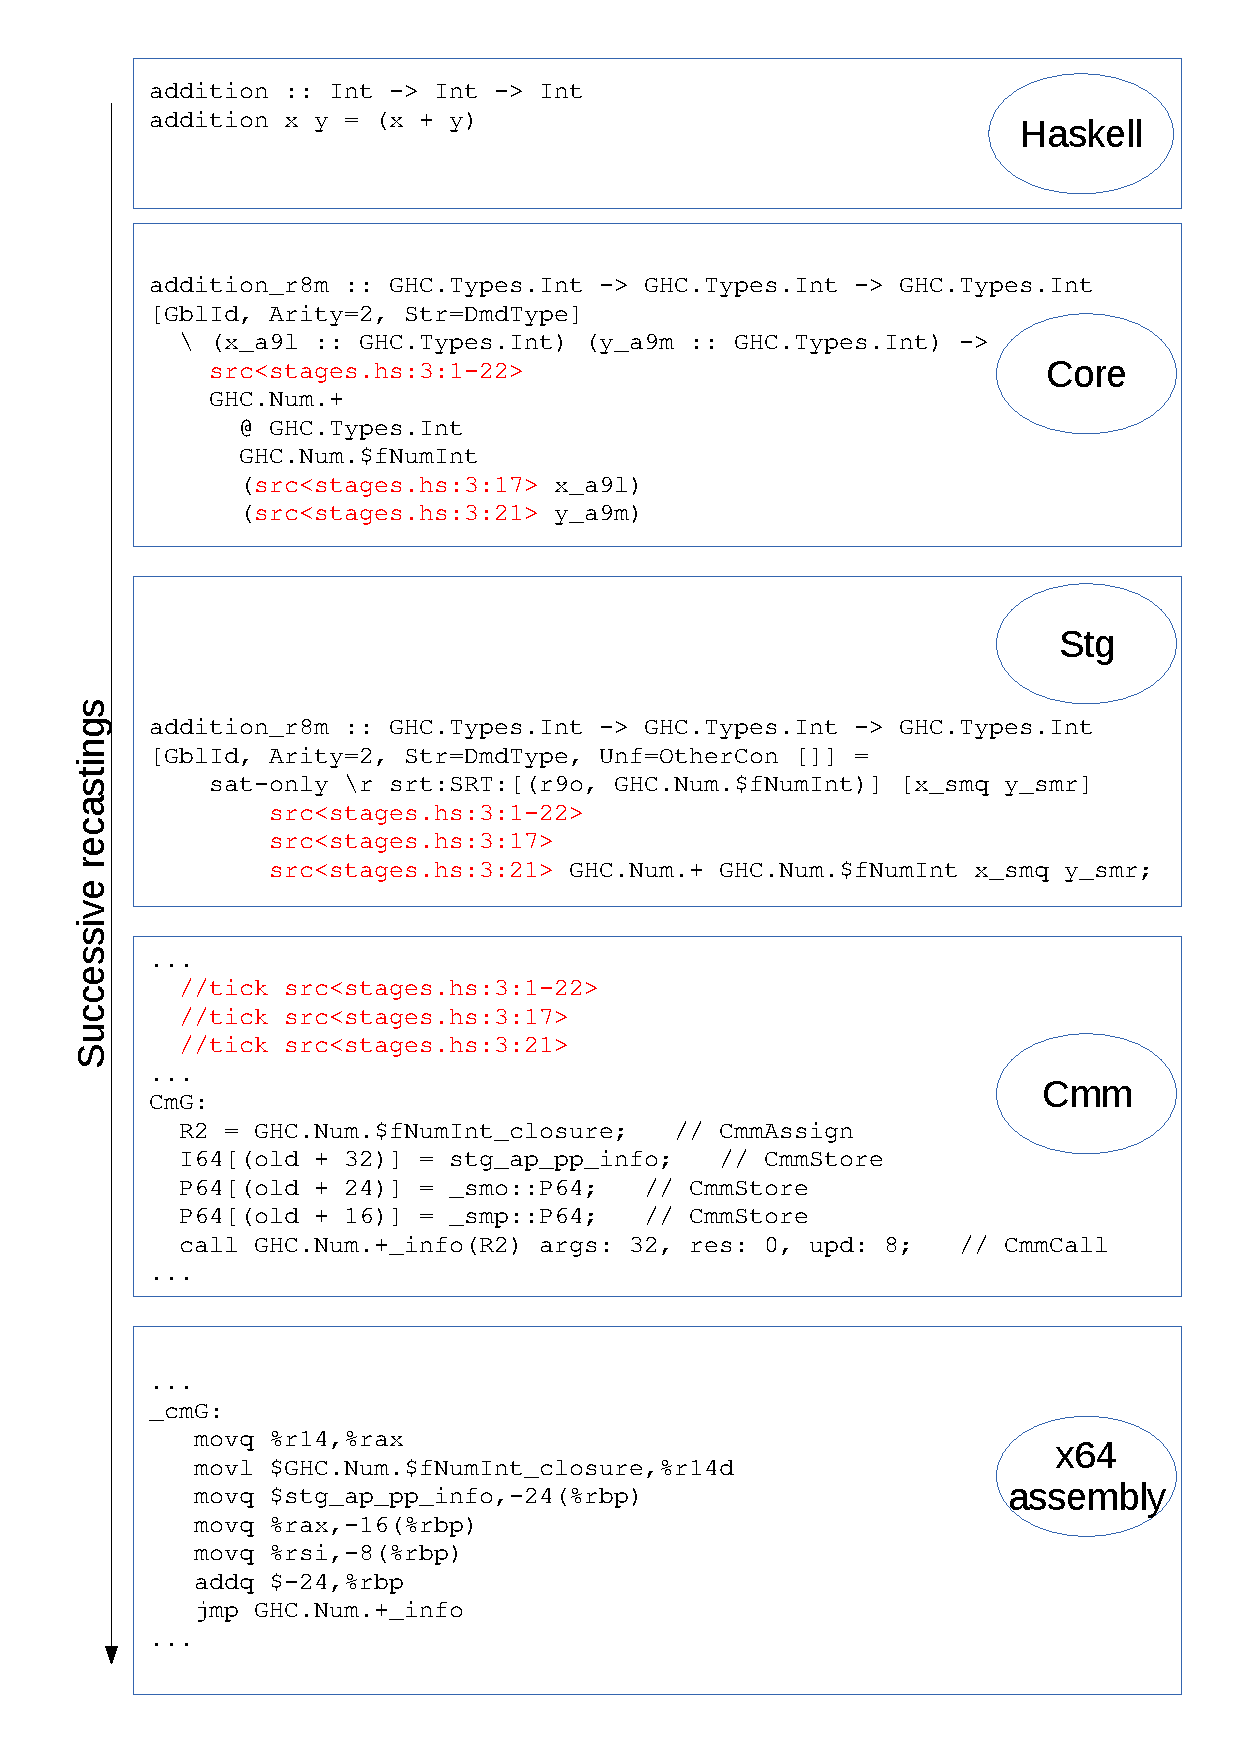
\includegraphics[width=2.2in]{fig/recastings_ticks}
  \end{frame}

  \begin{frame}
   \frametitle{What happened?}
  % trim=l b r t
   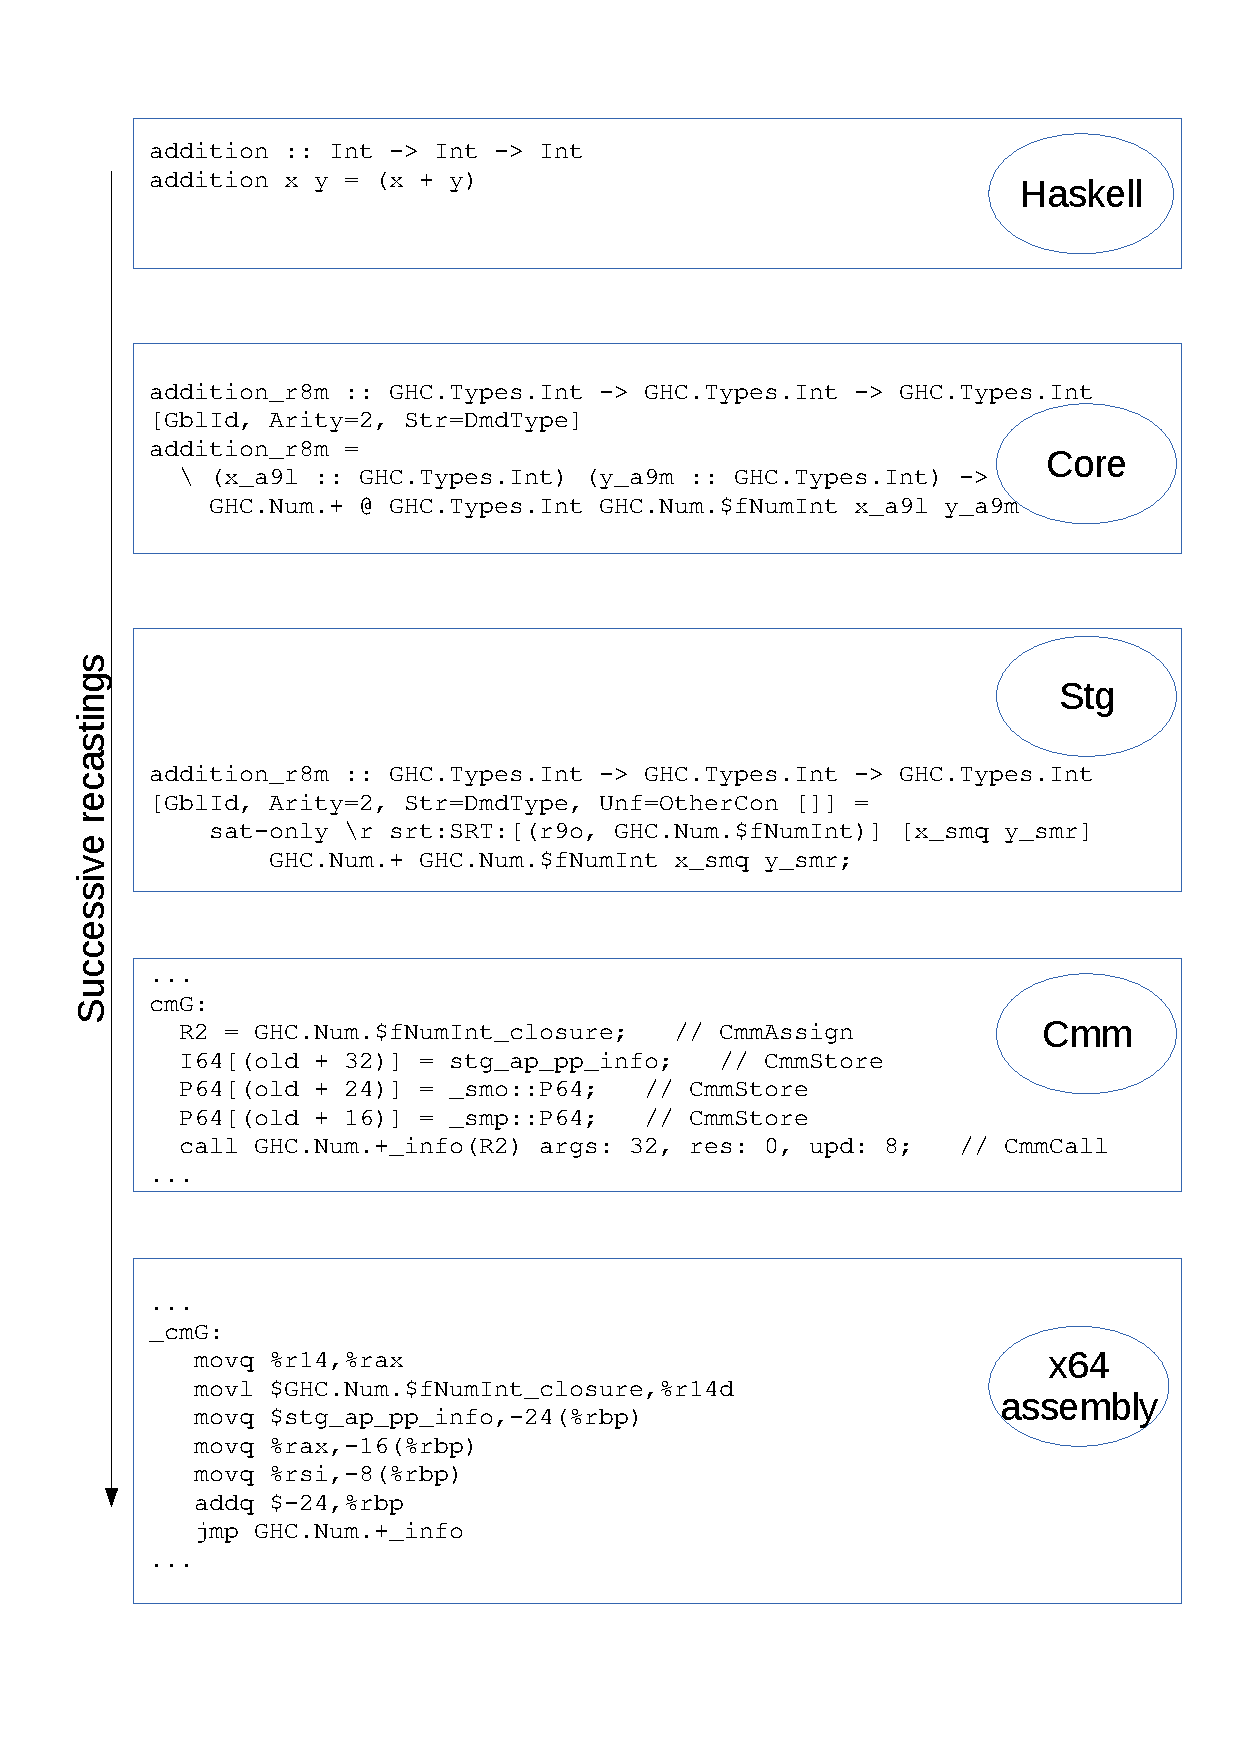
\includegraphics[trim=0 0.5in 0 7.8in, clip=true, width=2.2in]{fig/recastings}
   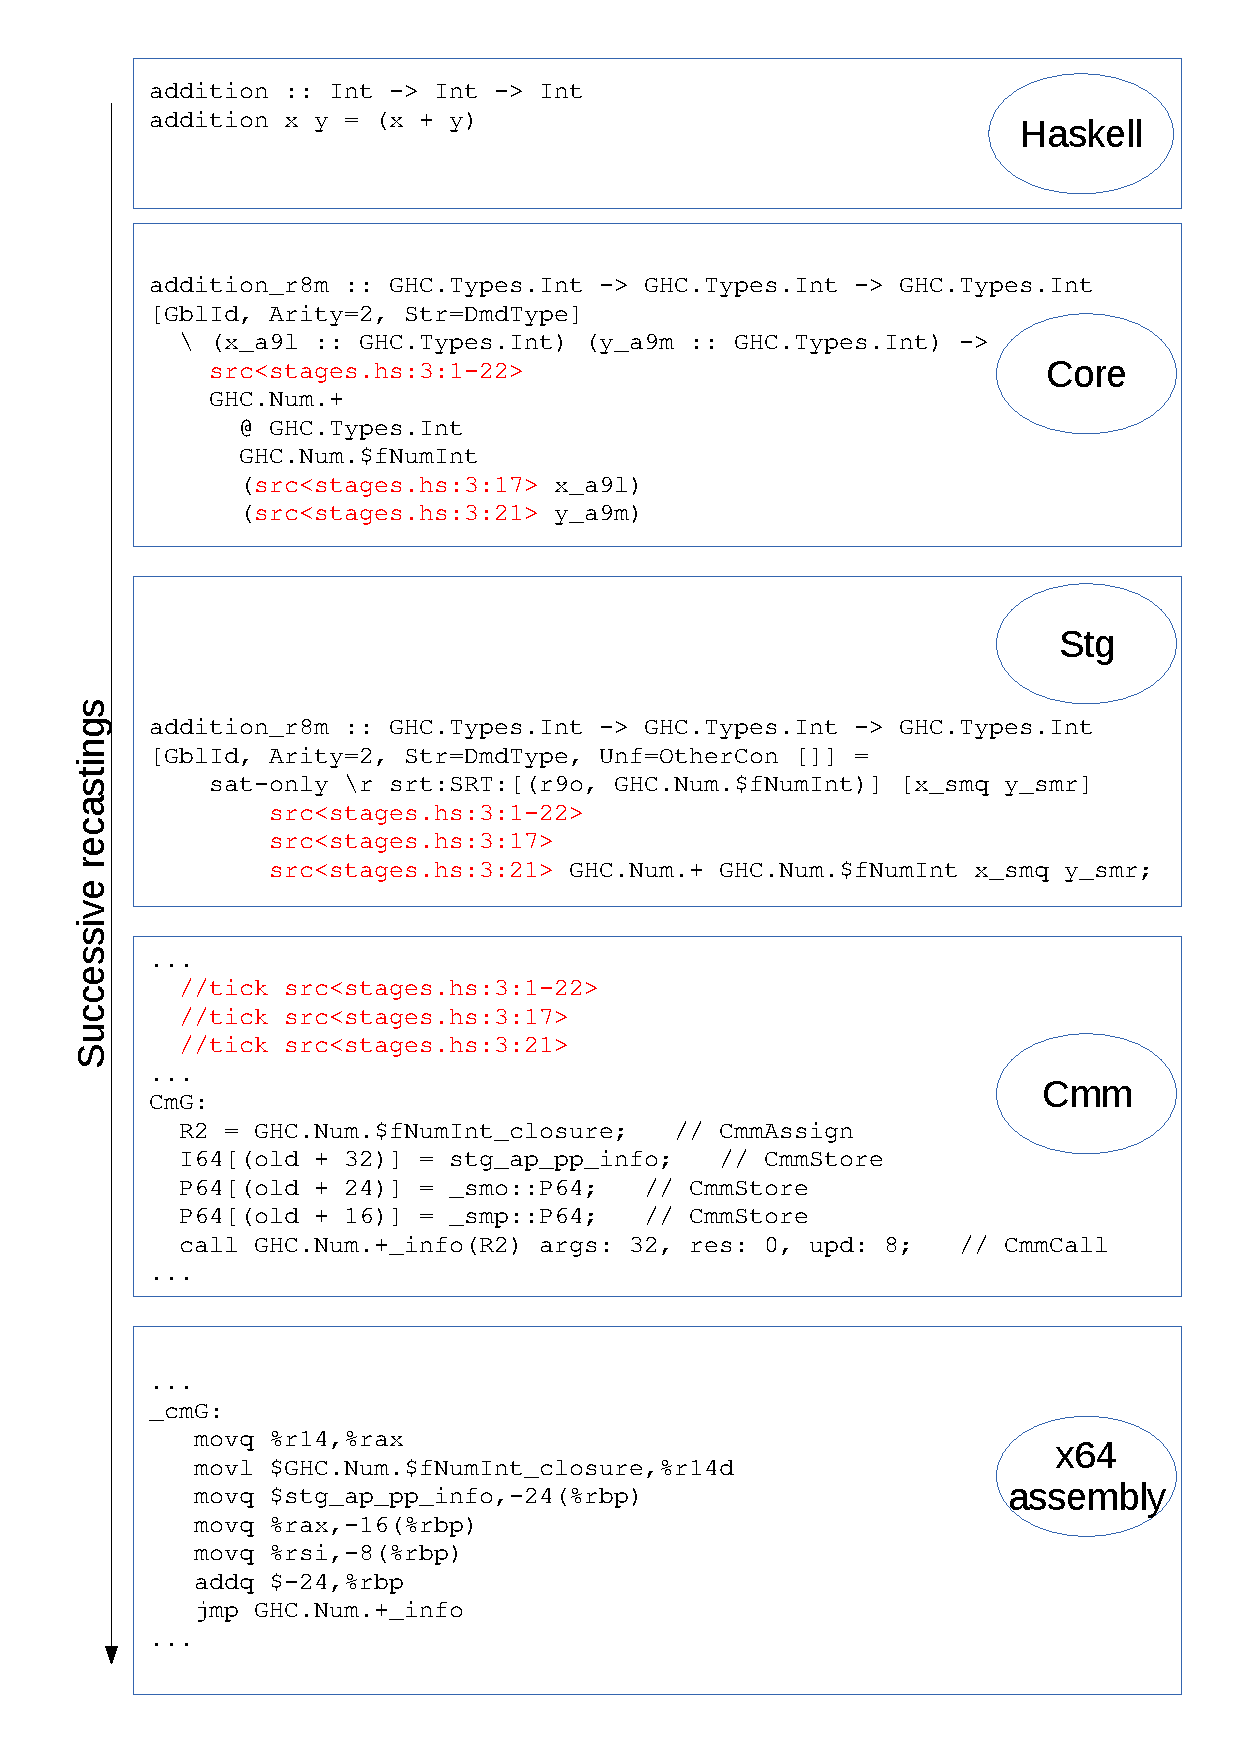
\includegraphics[trim=0 0 0 8.5in, clip=true, width=2.2in]{fig/recastings_ticks}
  \begin{itemize}
   \item Did we just drop the debug data we worked so hard for?
  \end{itemize}
  \end{frame}

  \begin{frame}
   \frametitle{This is a solved problem, of course!}
  \begin{itemize}
   \item <1-> DWARF to the rescue!
    \dwarfCode
   \item <2-> DWARF lives \emph{side by side} in another section of the binary.
     Therefore it does not interfere.
  \end{itemize}
  \end{frame}

\subsubsection{The Stack}

  \begin{frame}
   \frametitle{Introduction to the Execution Stack}
  \begin{itemize}
   \item <1-> GHC \emph{chooses} to implement Haskell with a stack.
   \item <2-> It does not use the normal ``C-stack''
   \item <3-> GHC maintains its own stack, we call it the \emph{execution stack}.
  \end{itemize}
  \end{frame}

  \begin{frame}
   \frametitle{Similar but not same}
  \begin{itemize}
   \item <1-> Unlike C, we do not push something on the stack when entering a function!
   \item <2-> Unlike C, we have cheap green threads, one stack per thread!
  \end{itemize}
  \end{frame}

  \begin{frame}
   \frametitle{What is on it then?}
  \begin{itemize}
   \item <1-> Recall this code:
     \caseCode
   \item <2-> How is this implemented? Let's think for a while \dots
   \item <3-> Aha! We can push a \emph{continuation} on the stack and jump to the code of \texttt{myBool}!
   \item <4-> We call this a \emph{case continuation}.
  \end{itemize}
  \end{frame}

\section{The breakthrough in August 2013}

  \begin{frame}
   \frametitle{Peter's demonstration}
  \begin{itemize}
   \item <1-> In August 2013 Peter Wortmann showed a proof of concept stack
     trace based on his work.
   \item <2-> My master thesis is entirely based on Peter's work.
  \end{itemize}
  \end{frame}

  \begin{frame}
   \frametitle{The stack trace \dots}
  \begin{itemize}
   \item For this Haskell code:
     \HaskellSTCode
  \end{itemize}
  \end{frame}

  \begin{frame}
   \frametitle{\dots is \emph{terrible}!}
  \begin{itemize}
   \item <1-> We get:
     \OriginalTraceCode
   \item <2-> We want:
     \IdealTraceCode
  \end{itemize}
  \end{frame}

\section{Contribution}

  \begin{frame}
   \frametitle{Then what did Arash do?}
  \begin{itemize}
   \item <1-> In addition to an unreadable stack trace, the time and memory
     complexity of stack reification can be improved.
   \item <2-> The stack reification in Peter Wortmann's demonstration is linear
     in time and memory.
   \item <3-> \emph{Obviously}, if you throw a stack and then print it. It can
     not be worse than linear in time.
   \item <4-> \emph{But}, if you throw a stack and do \emph{not} print it, a
     reification that is done \emph{lazily} would be done in constant time.
  \end{itemize}
  \end{frame}

  \begin{frame}
   \frametitle{So the problems to tackle are:}
  \begin{itemize}
   \item <1-> Make stack traces readable
   \item <2-> Make reification optimal complexity wise
   \item <3-> Add a Haskell interface to this
  \end{itemize}
  \end{frame}

\subsection{Using the execution stack}

  \begin{frame}
   \frametitle{We must understand the stack}
  \begin{itemize}
   \item <1-> What is on the stack?
   \item <2-> The C stack just have return addresses and local variables.
   \item <3-> The Haskell stack have many different kinds of members. Case
     continuations, update frames, catch frames, stm frames, stop frame,
     underflow frames etc.
   \item <4->
     
\includegraphics[width=3.2in]{fig/junkyard-gang}
  \end{itemize}
  \end{frame}

  \begin{frame}
   \frametitle{Update frames}
  \begin{itemize}
   \item <1-> Consider
     \obviouslyThunkCode
   \item <2-> In GHC, thunks are memoized by default
   \item <3-> This is done by update frames on the stack
   \item <4-> Details omitted in interest of time
  \end{itemize}
  \end{frame}

  \begin{frame}
   \frametitle{New policy for reifying update frames}
  \begin{itemize}
   \item <1-> So instead of saying that we have an update frame, refer to its
     updatee.
  \end{itemize}
     \improvedTraceCode
  \end{frame}


  \begin{frame}
   \frametitle{Other frames}
  \begin{itemize}
   \item <1-> Many of the frames are interesting. But the most common one is
     probably case continuations, which luckily are unique and therefore useful
     when applying \texttt{getDebugInfo}
  \end{itemize}
  \end{frame}

\subsection{Reifying efficiently}

  \begin{frame}
   \frametitle{The problem}
  \begin{itemize}
   \item <1-> On a crash, the stack is unwounded and the stack reified
   \item <1-> Control is passed to the first catch frame on the stack
   \item <2-> Imagine the function 
     \catchWithStackCode
   \item <2-> What can \texttt{Stack} be?
   \item <2-> Can it really be lazily evaluated?
   \item <3-> We have to be really careful, the stack is a mutable data structure!
  \end{itemize}
  \end{frame}

  \begin{frame}
   \frametitle{One idea}
  \begin{itemize}
   \item <1-> Internally, the execution stack is a \emph{chunked linked list}.
   \item <1-> What if we \emph{freeze} the stack and continue our stack in a new chunk?
   \item <2->
     \includegraphics[height=2.2in]{build/fig/stack}
     \includegraphics[height=2.2in]{build/fig/stack-new}
  \end{itemize}
  \end{frame}

\subsection{Haskell interface}

  \begin{frame}
   \frametitle{Why an Haskell interface?}
  \begin{itemize}
   \item <1-> Compare
     \begin{itemize}
       \item \texttt{gdb} style of stack traces
       \item Catching an exception with the stack trace 
     \end{itemize}
   \item <2-> The latter is \emph{much} more powerful since we have control
     over it in Haskell land
   \item <3-> We can:
     \begin{itemize}
       \item Print to screen
       \item Email it
       \item Choose to handle the exception based on if frame X is present on
     \end{itemize}
   \item <4-> Definitely a requirement for software running in production
  \end{itemize}
  \end{frame}


  \begin{frame}
   \frametitle{The final Haskell API}
  \begin{itemize}
   \item <1-> Meh
     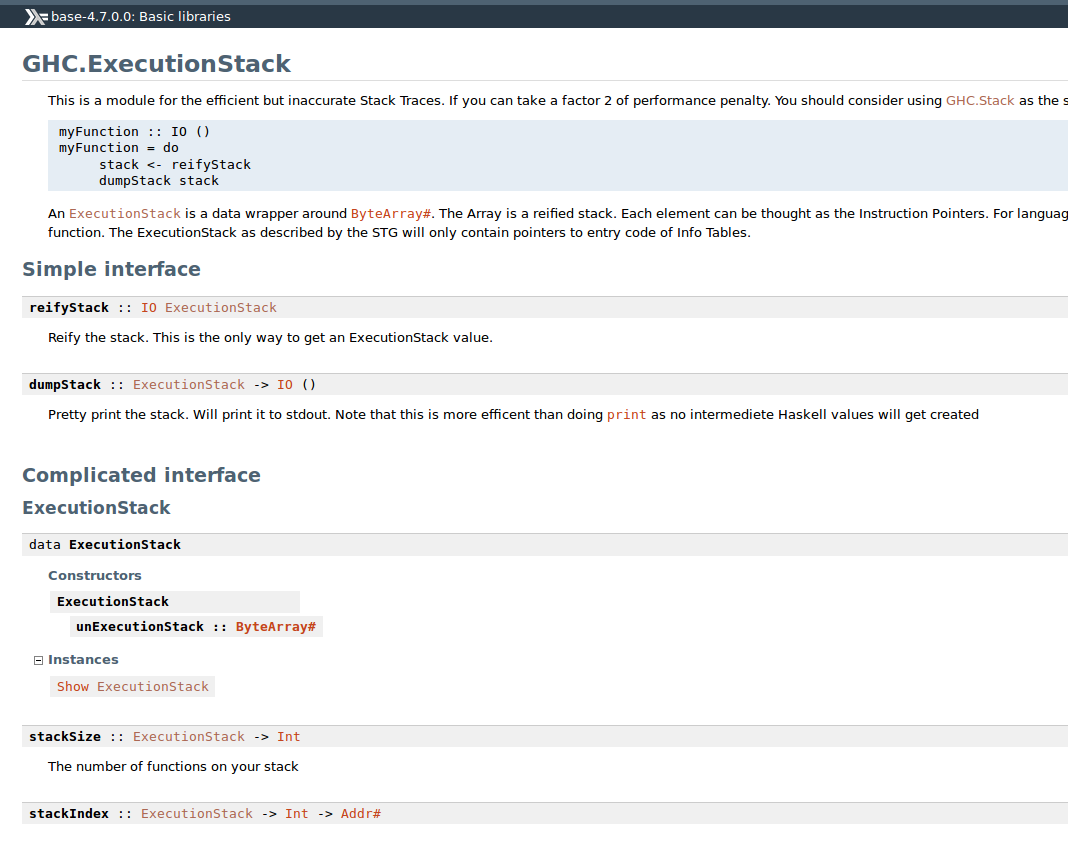
\includegraphics[width=3.2in]{fig/haddock-screenshot}
  \end{itemize}
  \end{frame}

\section{Conclusion}

  \begin{frame}
   \frametitle{Final remarks}
  \begin{itemize}
   \item <1-> It seems possible to create an efficient first-class value of the
     execution stack that is available post mortem. If my ideas work out this
     will be \emph{amazing}
   \item <1-> This work will not be so super-useful unless it incorporates with
     exceptions that Haskell is not aware of, like segmentation faults. Think
     foreign function calls and Haskell code like: \mint{haskell}|unsafeWrite v 1000000000 (0 :: Int)|
  \end{itemize}
  \end{frame}

  \begin{frame}
   \frametitle{Demo!}
  \begin{itemize}
   \item Demo!!
  \end{itemize}
  \end{frame}

\end{document}
